\begin{figure}[H]
	\centering
	\begin{minipage}{\linewidth}
		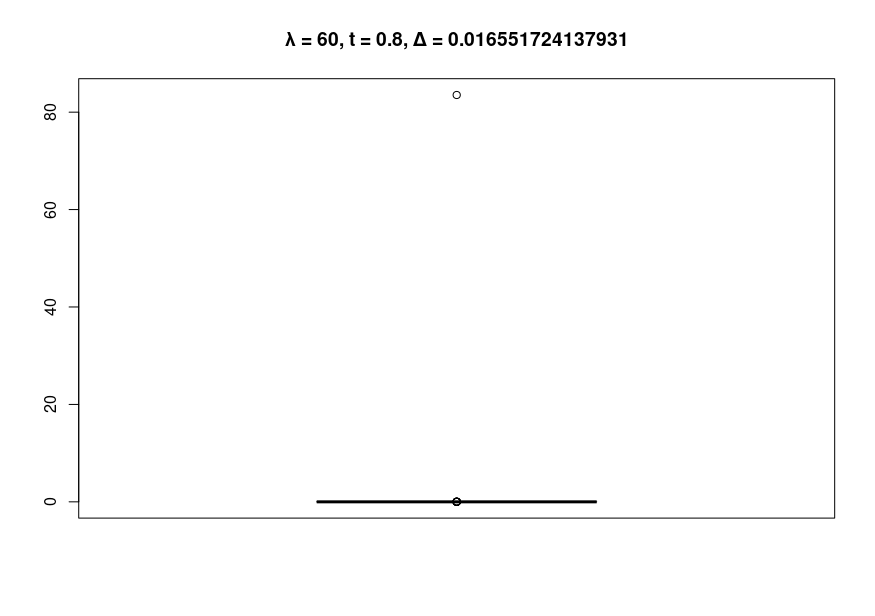
\includegraphics[width=0.43\textwidth]{Images/indiv_vs_glob/qq160.png}
		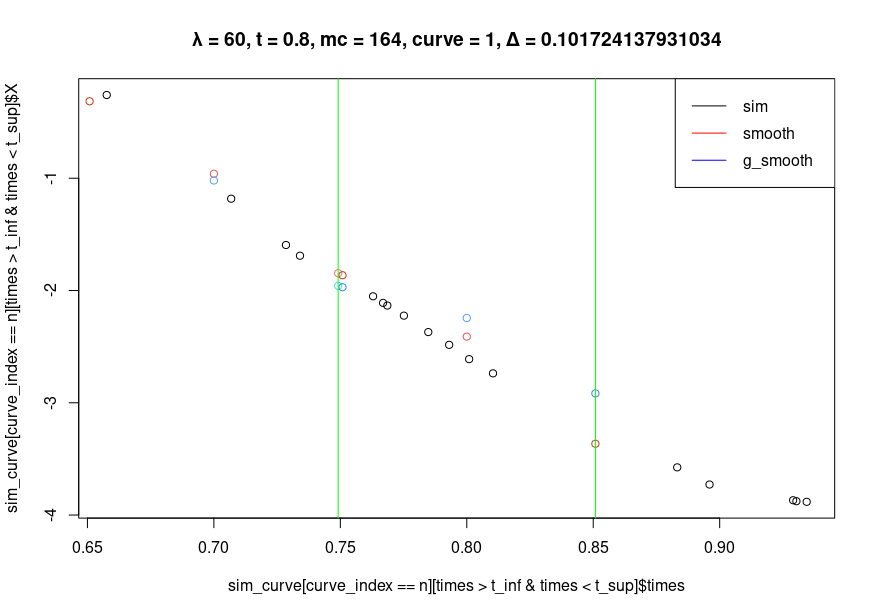
\includegraphics[width=0.43\textwidth]{Images/indiv_vs_glob/lbd60mc164c1.png}
	\end{minipage}

	\begin{minipage}{\linewidth}
		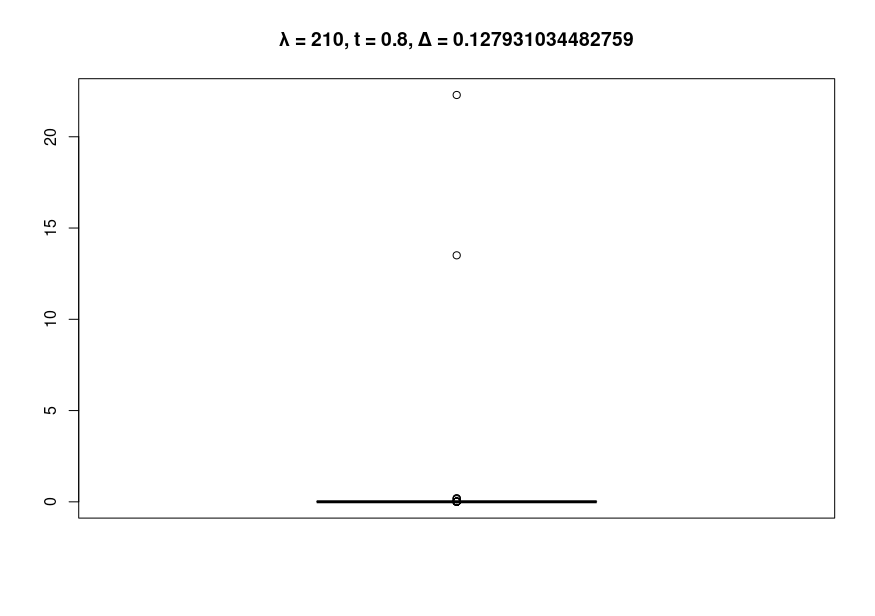
\includegraphics[width=0.43\textwidth]{Images/indiv_vs_glob/qq210.png}
		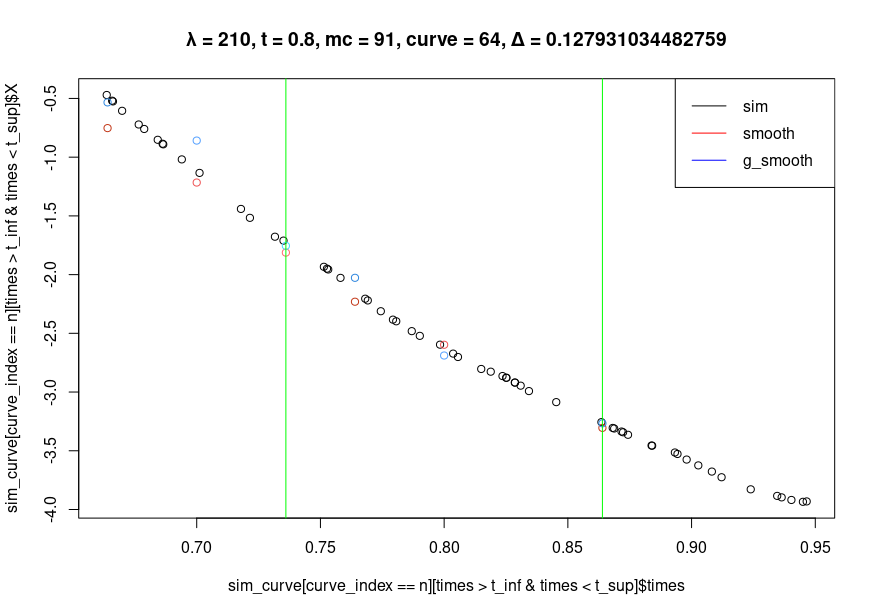
\includegraphics[width=0.43\textwidth]{Images/indiv_vs_glob/lbd210_mc91_c64.png}
	\end{minipage}
	\caption{Distribution des risques et aperçu d'une courbe pour un échantillon de Monte-Carlo extrême sur le risque euclidien.}
	\label{fig:dist_R_eucl_curves}
\end{figure}

\begin{figure}[H]
	\centering
	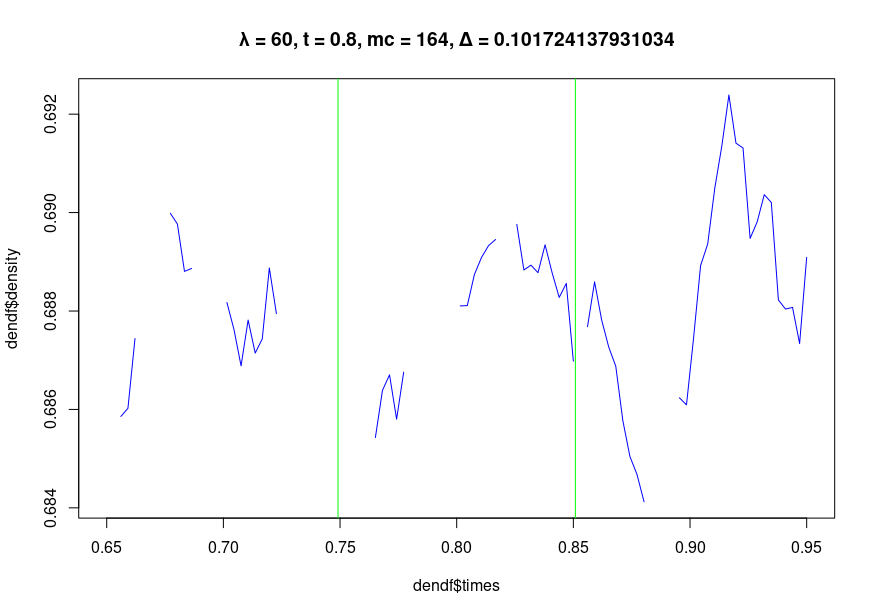
\includegraphics[width=0.7\textwidth]{Images/indiv_vs_glob/Tdensity_lbd60_mc164.png}
	\caption{Densité de points observés sur $[0.65, 0.95]$ pour $\lambda = 60$ sur un échantillon de Monte-Carlo extrême, en un $\Delta$ problématique.}
	\label{fig:den_ex}
\end{figure}


\begin{figure}[H]
	\centering
	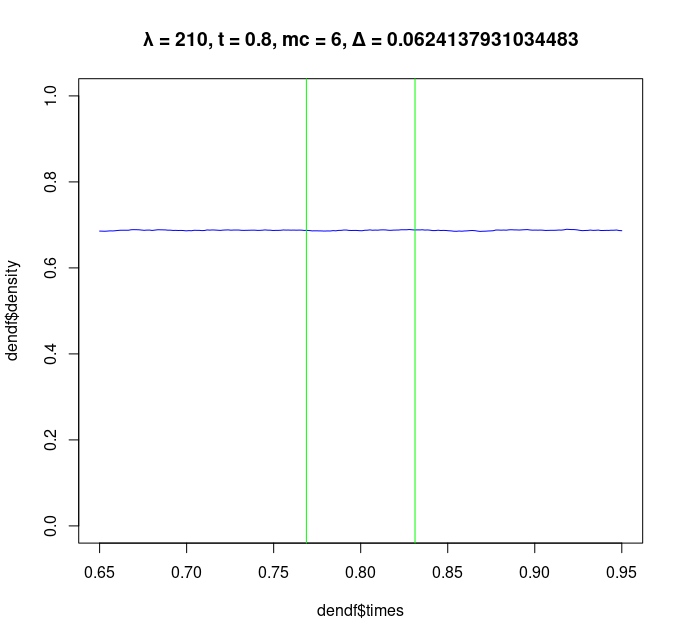
\includegraphics[width=0.7\textwidth]{Images/indiv_vs_glob/worst_210_67_mc6.png}
	\caption{Densité des points observés correspondant à la courbe présentée sur la figure \ref{fig:dist_R_eucl_curves}.}
	\label{fig:den_counterex}
\end{figure}

\largeskip

\warn{

\bigskip\centering

Dans l'ensemble des graphes suivants se trouve une erreur de labélisation des graphes : La métrique $\mathcal R$ considérée est bel et bien la norme euclidienne \textbf{au carré} $\mathcal R ( \Theta , \Delta) = \mathds E {\distnorme 2 {\widehat \Theta} {\widetilde \Theta}}^2$. De même que la norme relative considérée est la norme relative \texbf{au carré} $\mathcal R ( \Theta , \Delta) = \mathds E \displaystyle \frac{{\distnorme 2 {\widehat \Theta} {\widetilde \Theta}}^2}{\norme 2 {\widetilde{\Theta}}}$

\bigskip

}

\begin{figure}[H]
	\centering

	\textbf{avec extrêmes : global}

	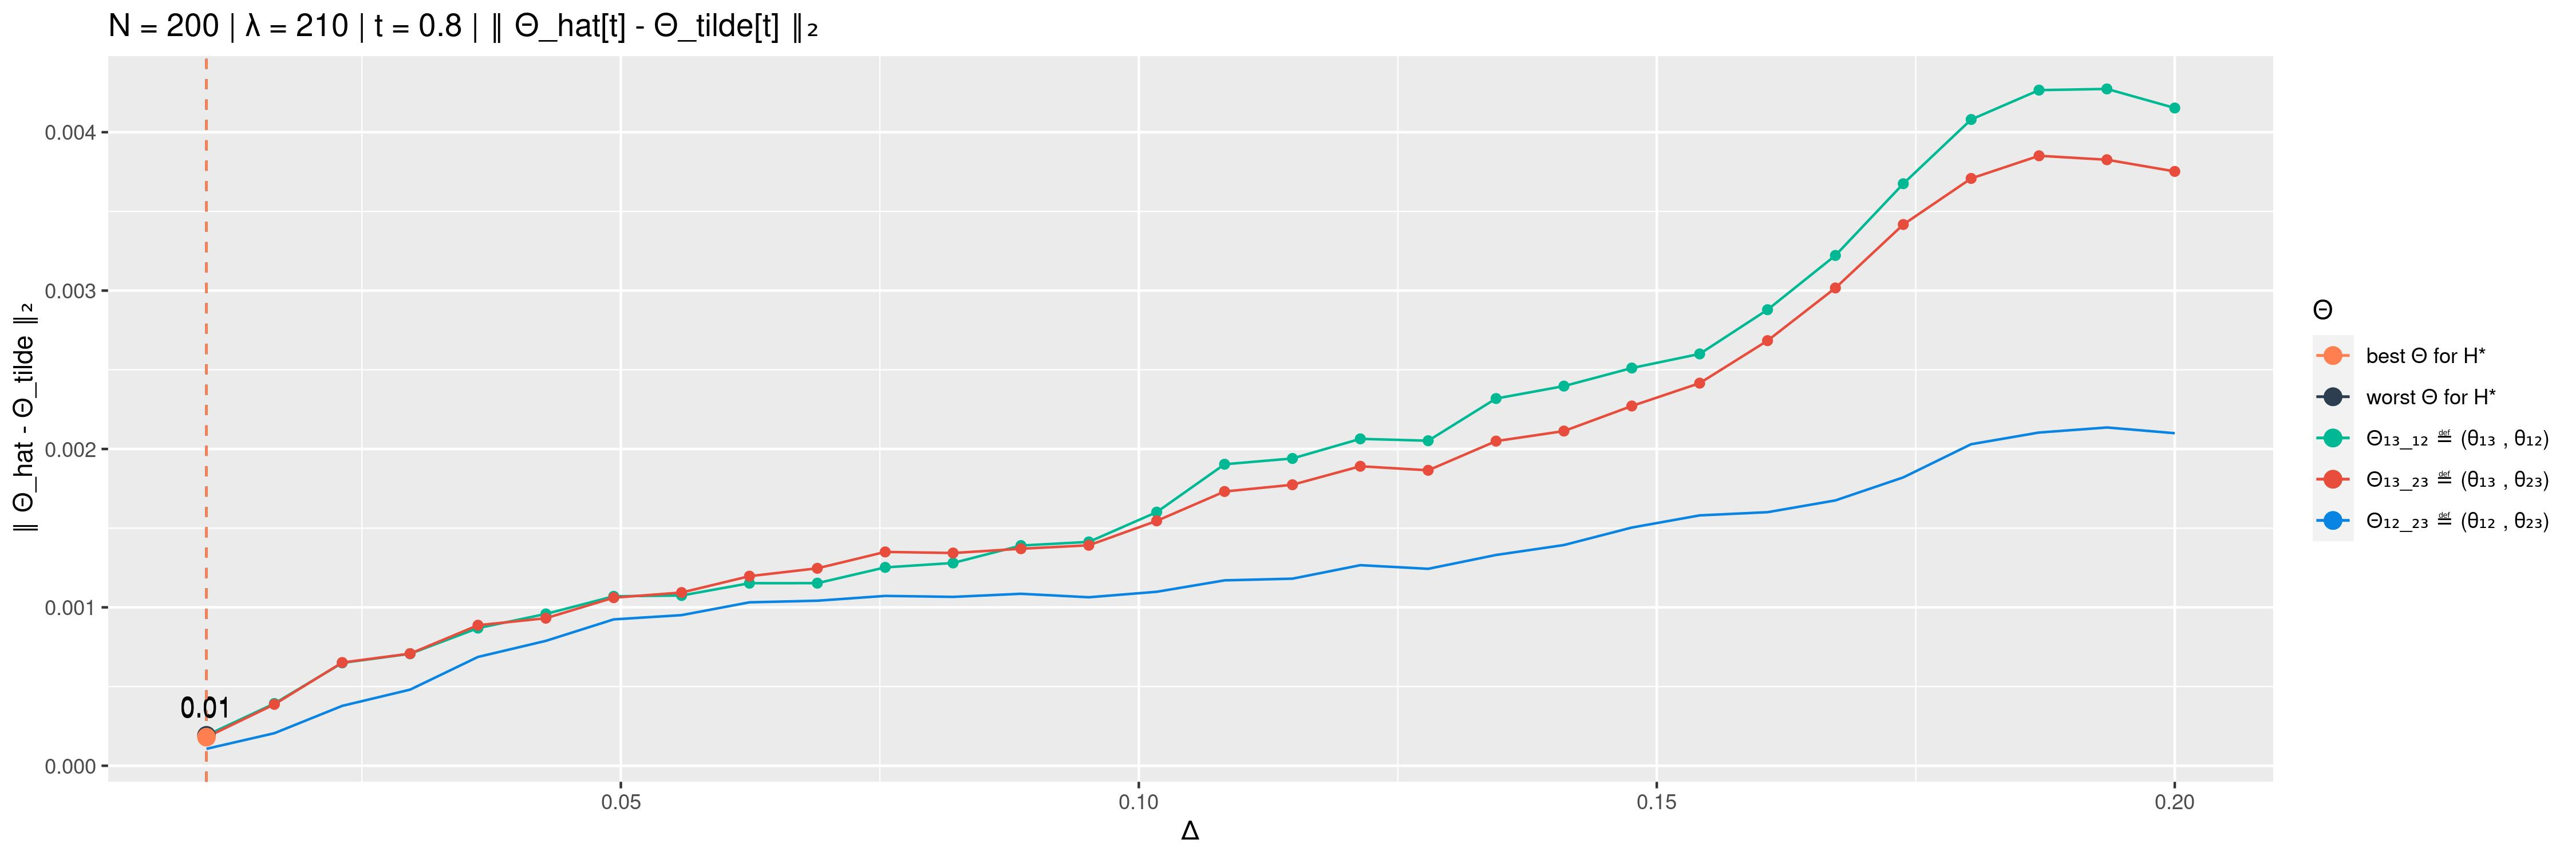
\includegraphics[width=0.9\textwidth]{Images/indiv_glob_img/compare/210_regular/all_glob.jpg}

	\textbf{avec extrêmes : individuel}

	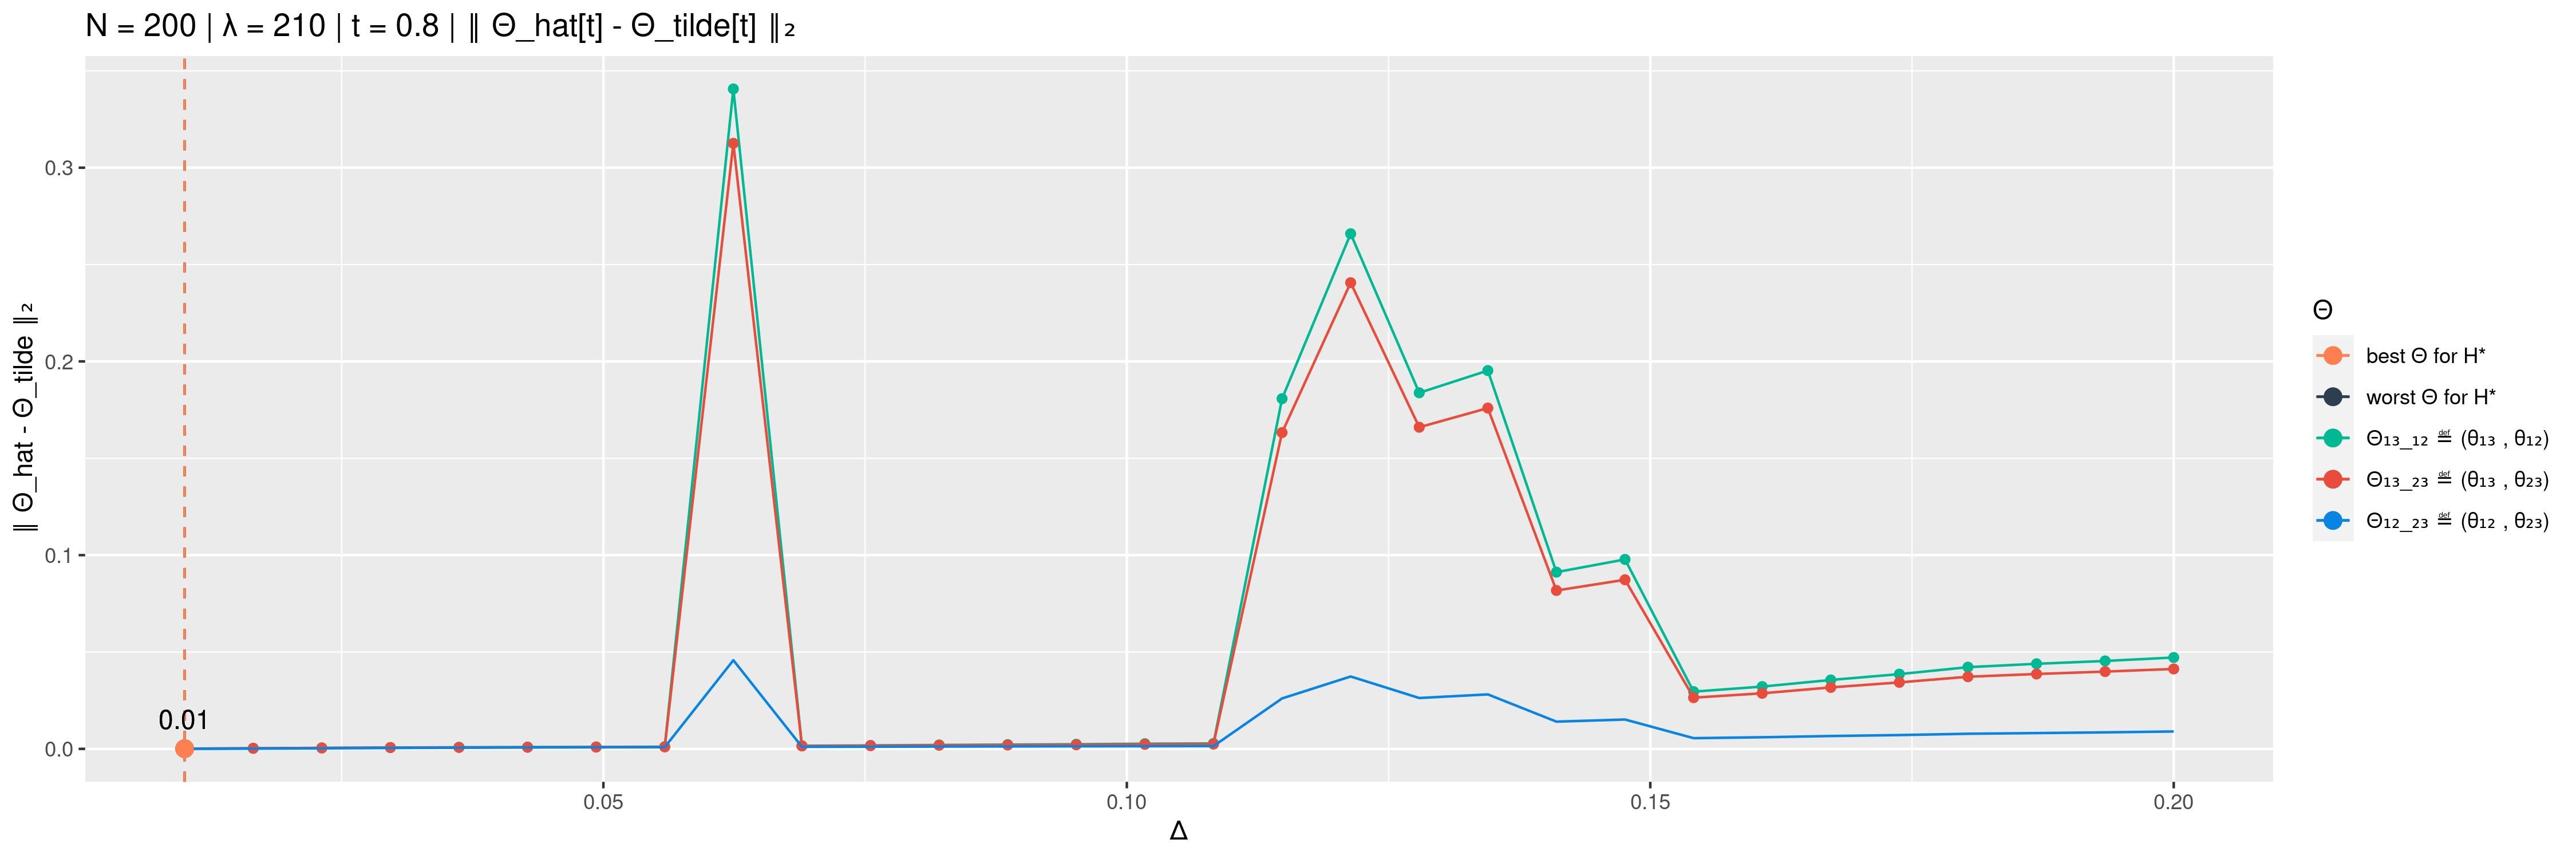
\includegraphics[width=0.9\textwidth]{Images/indiv_glob_img/compare/210_regular/all.jpg}

	\textbf{sans extrêmes : global} (- top 2\%)
	% TODO : changer d image : mauvais N, prendre N=200
	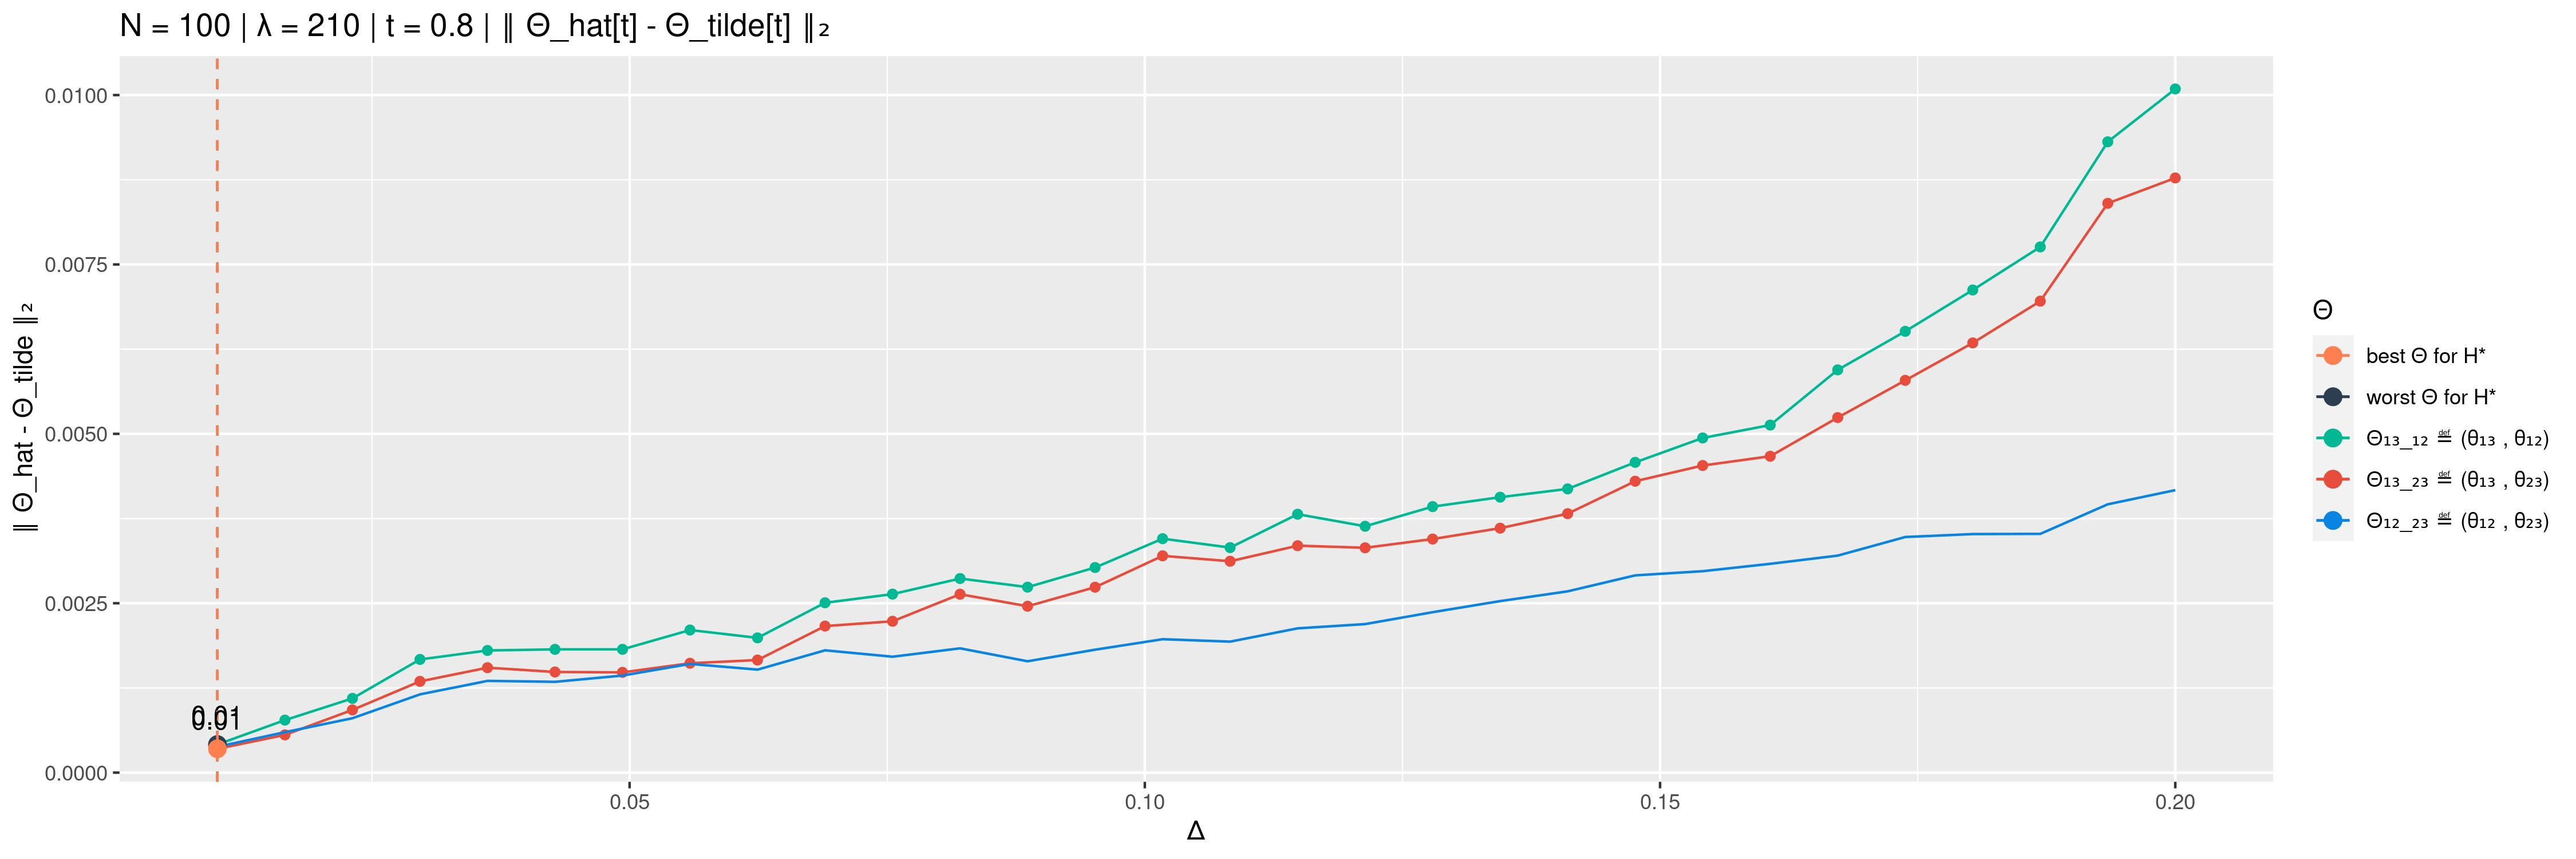
\includegraphics[width=0.9\textwidth]{Images/indiv_glob_img/compare/210_regular/no_xtrm_glob.jpg}

	\textbf{sans extrêmes : individuel} (- top 2\%)

	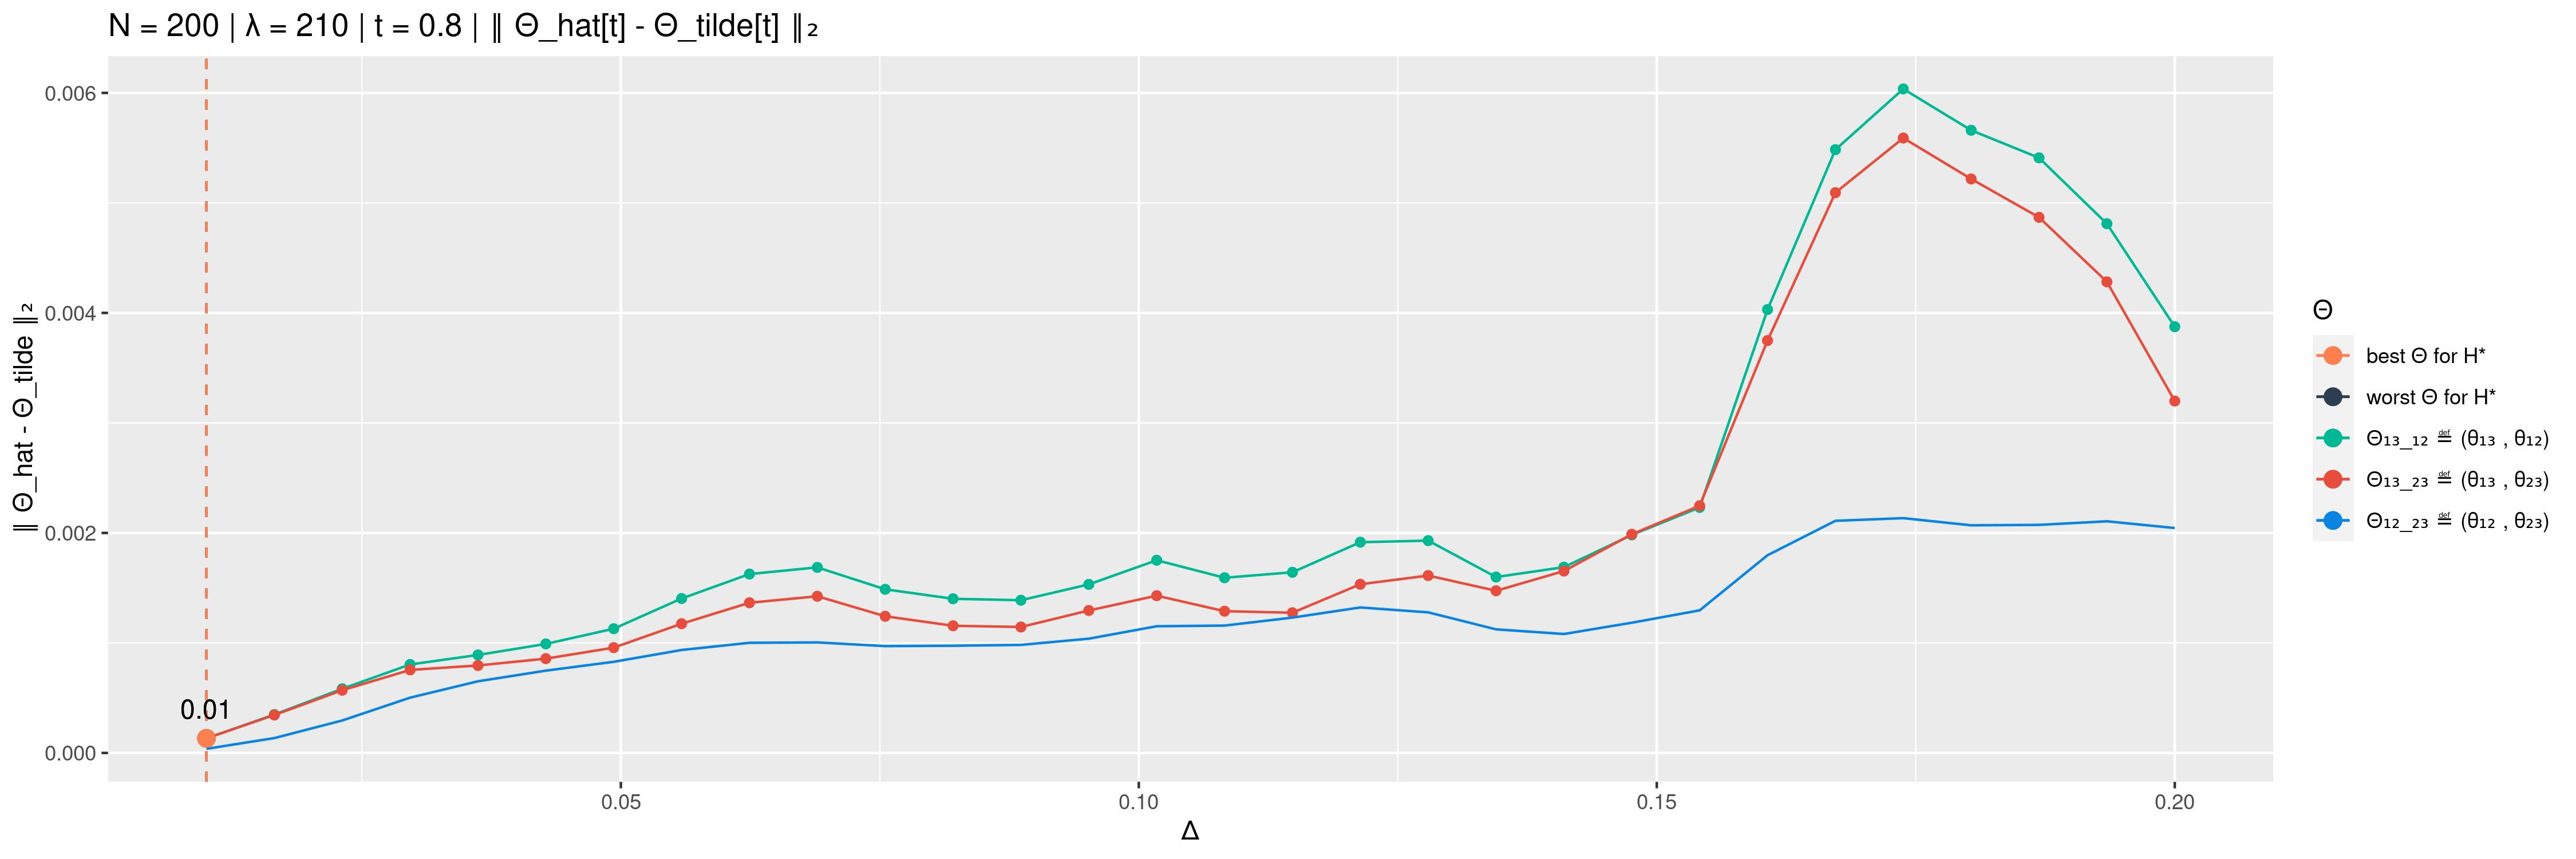
\includegraphics[width=0.9\textwidth]{Images/indiv_glob_img/compare/210_regular/no_xtrm.jpg}


	\caption{Risque Euclidien pour $N=200$, $\lambda=210$ en un point régulier selon la méthode utilisée pour la fenêtre de lissage}
	\label{fig:compare_xtrm_2}
\end{figure}

\begin{figure}[H]
	\centering
	\textbf{ H = 0.51 }

	Sparse :

	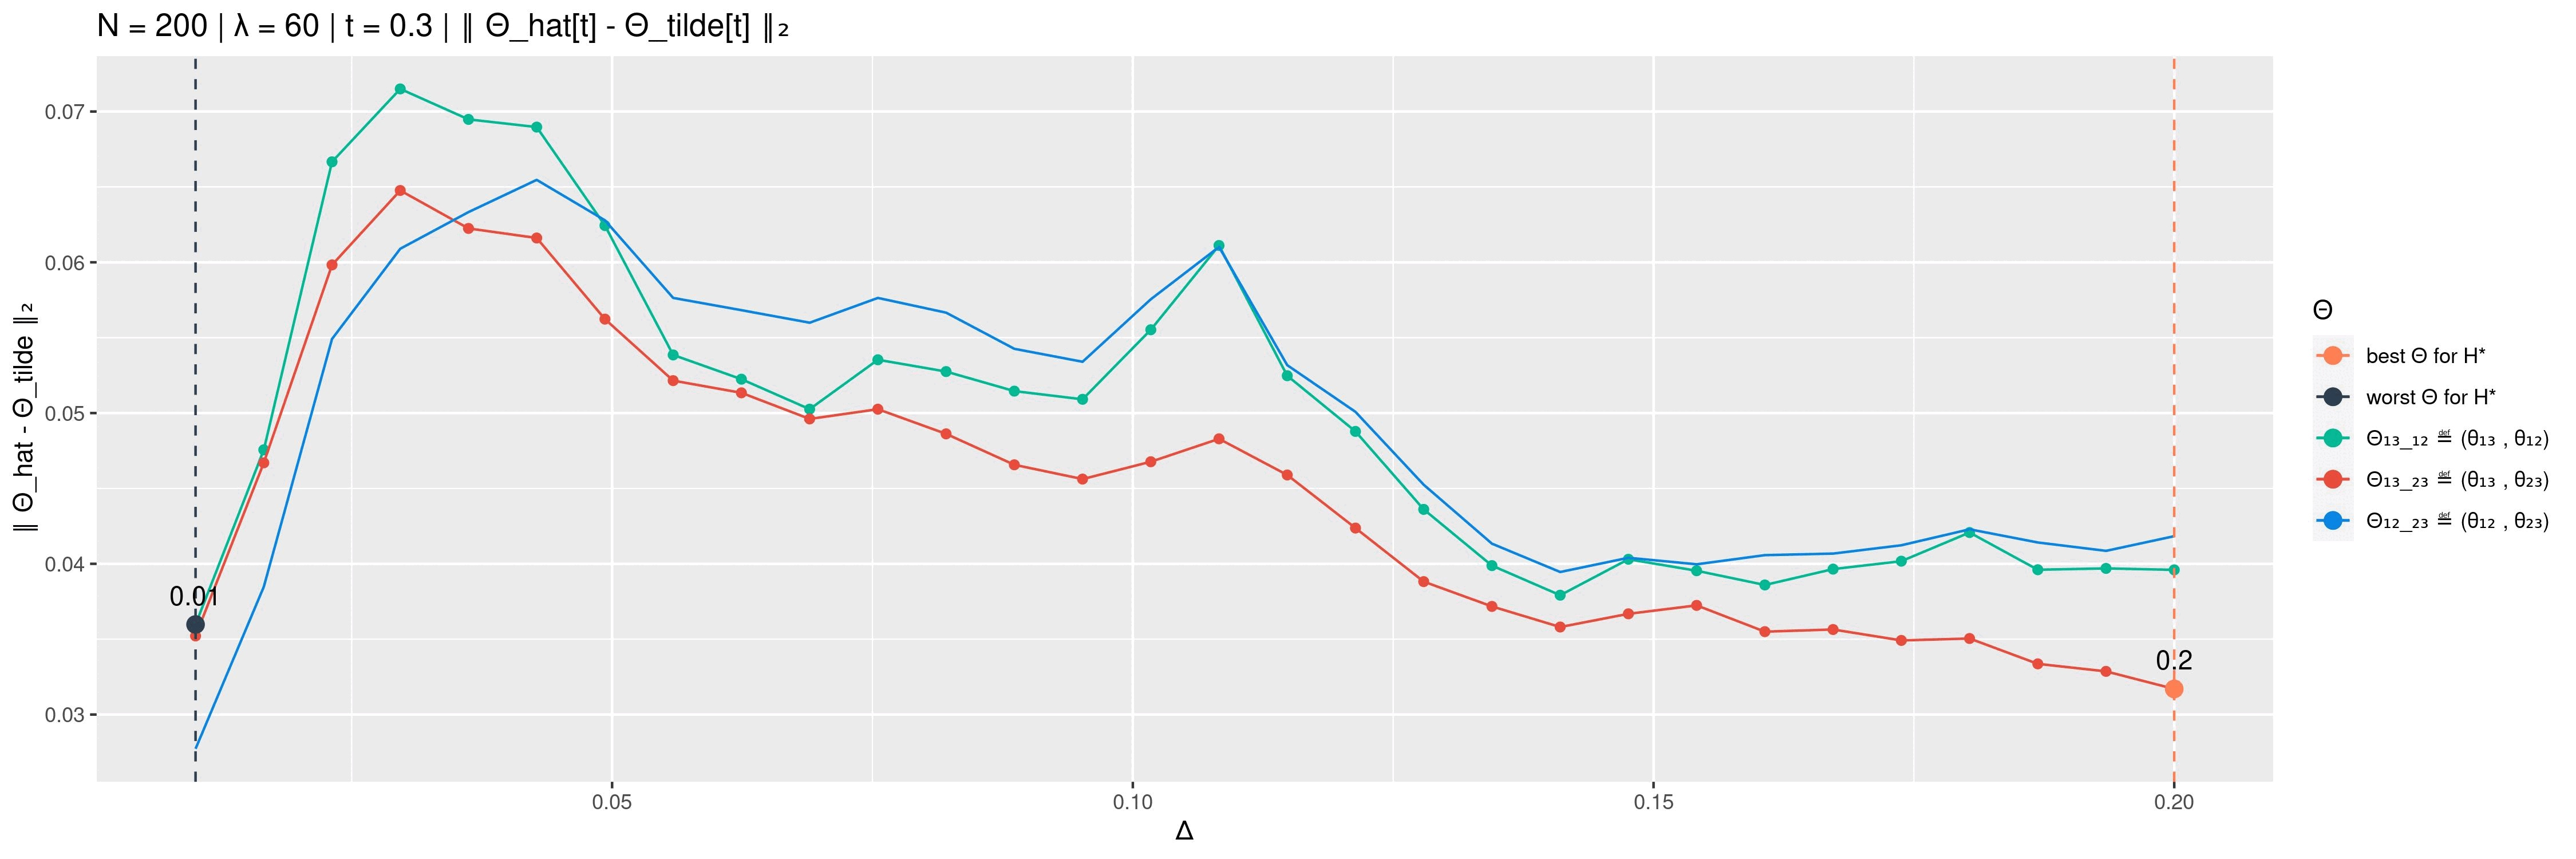
\includegraphics[width=0.8\textwidth]{Images/risque/N200_t0.3_lbd60.jpg}

	Dense :

	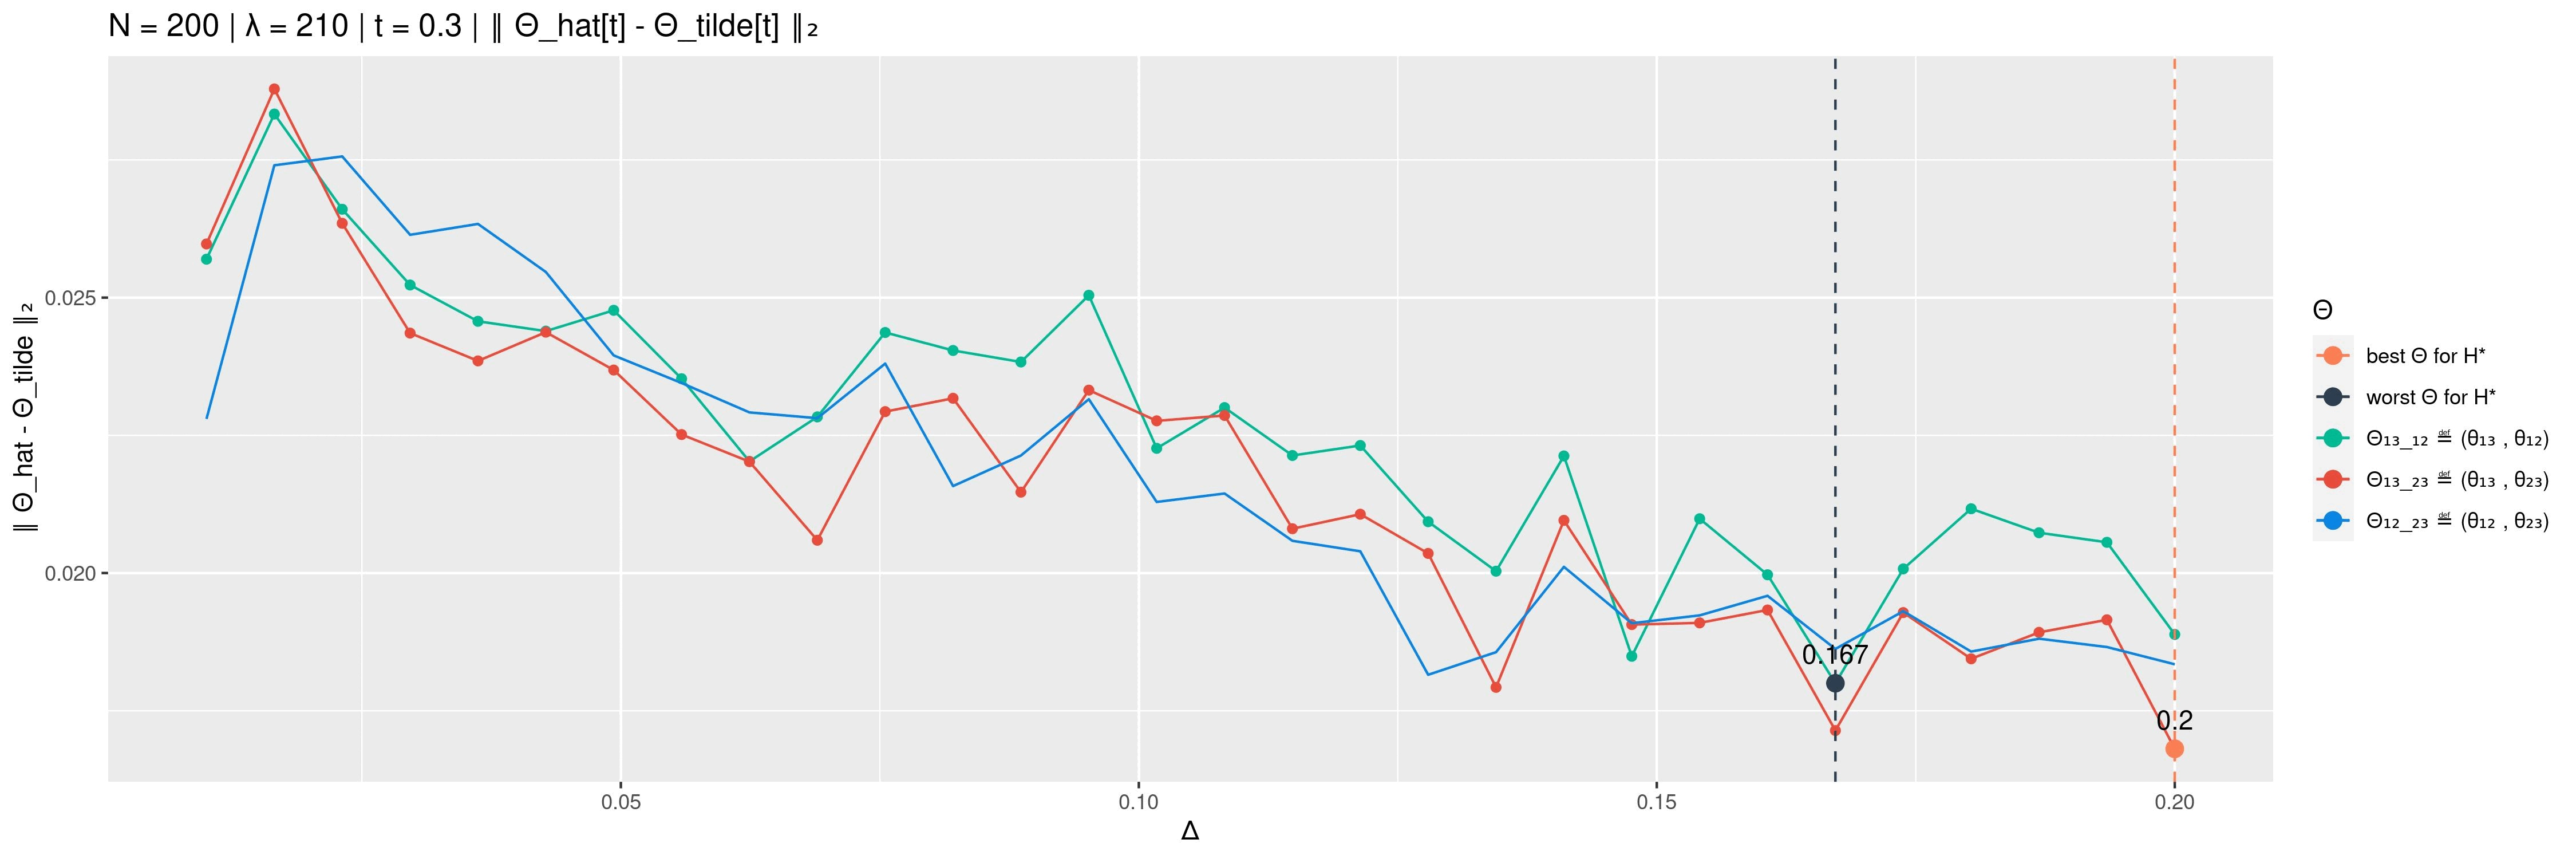
\includegraphics[width=0.8\textwidth]{Images/risque/N200_t0.3_lbd210.jpg}
\end{figure}

\begin{figure}[H]
	\centering
	\textbf{ H = 0.6 }

	Sparse :

	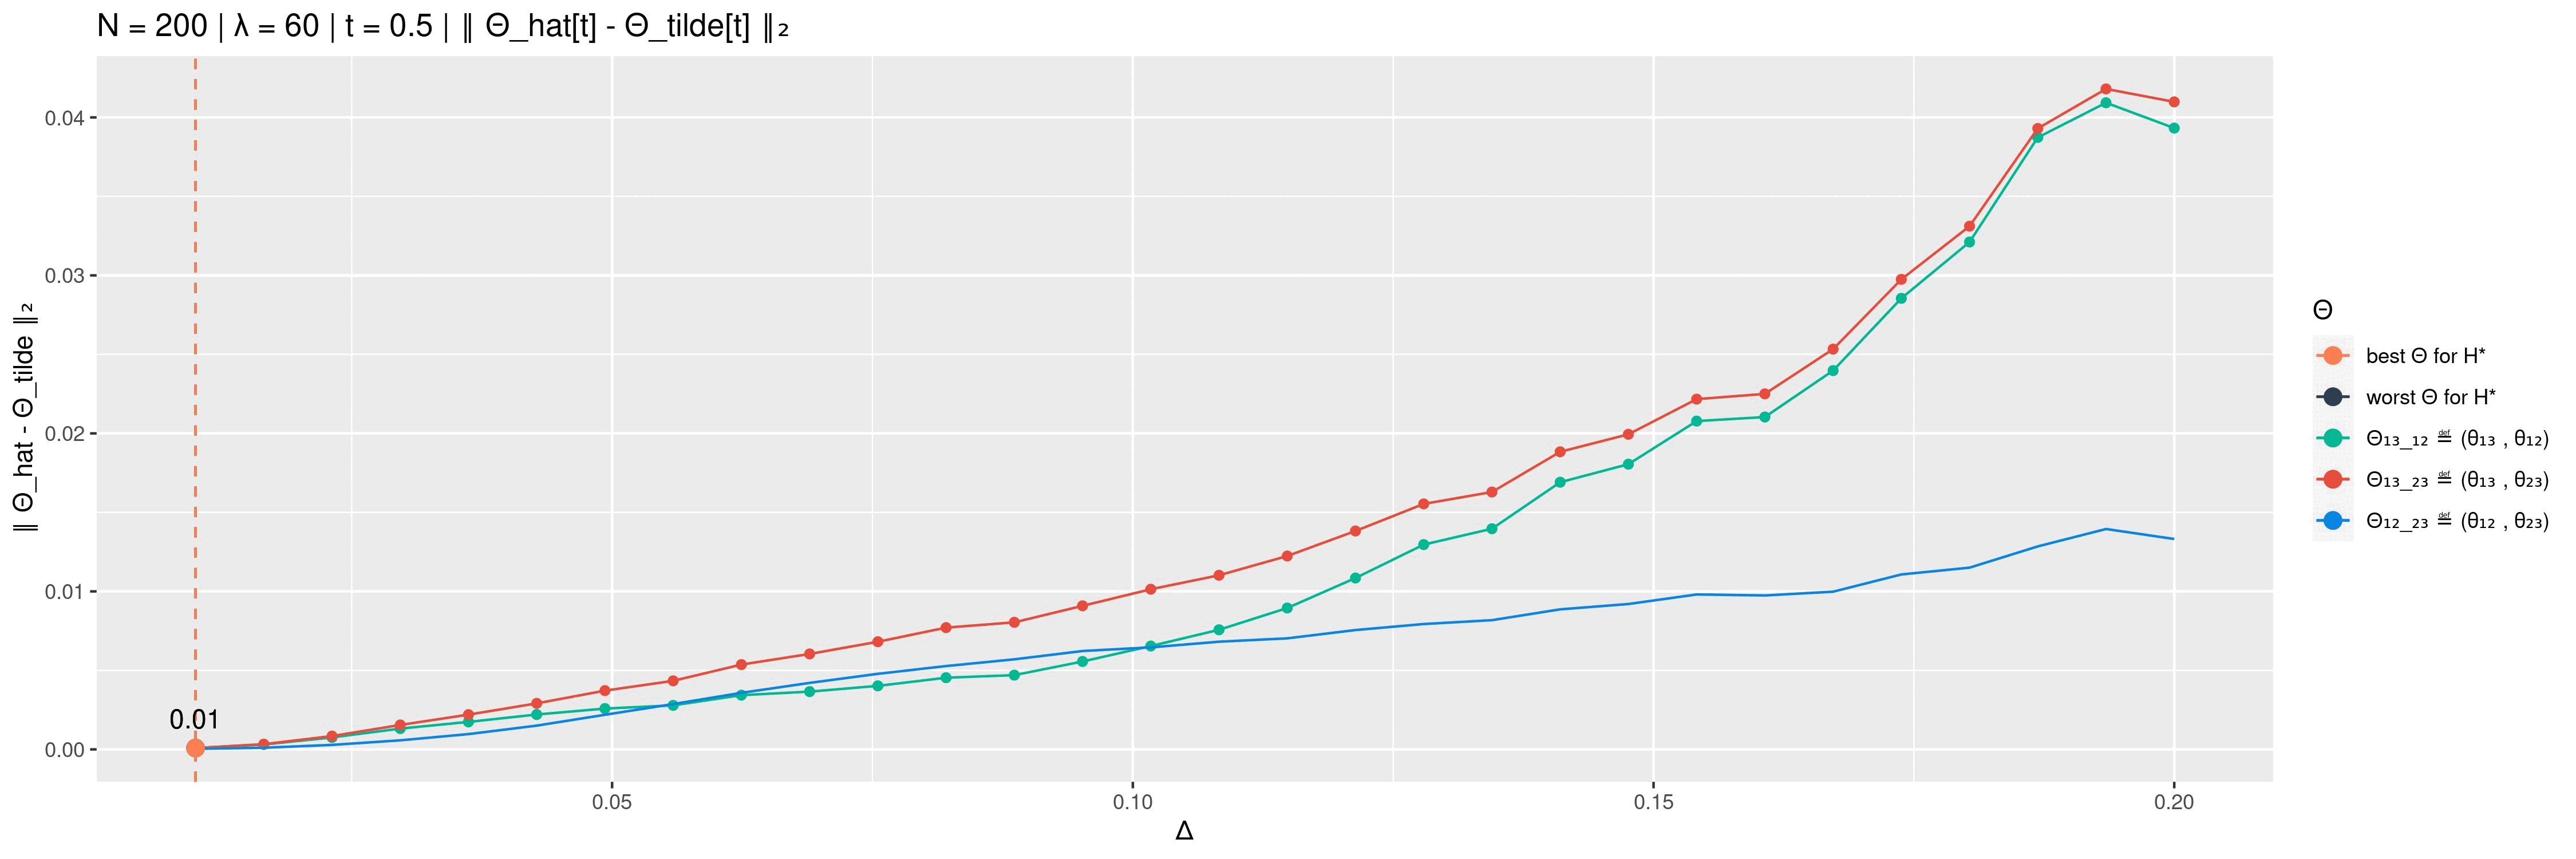
\includegraphics[width=0.8\textwidth]{Images/risque/N200_t0.5_lbd60.jpg}

	Dense :

	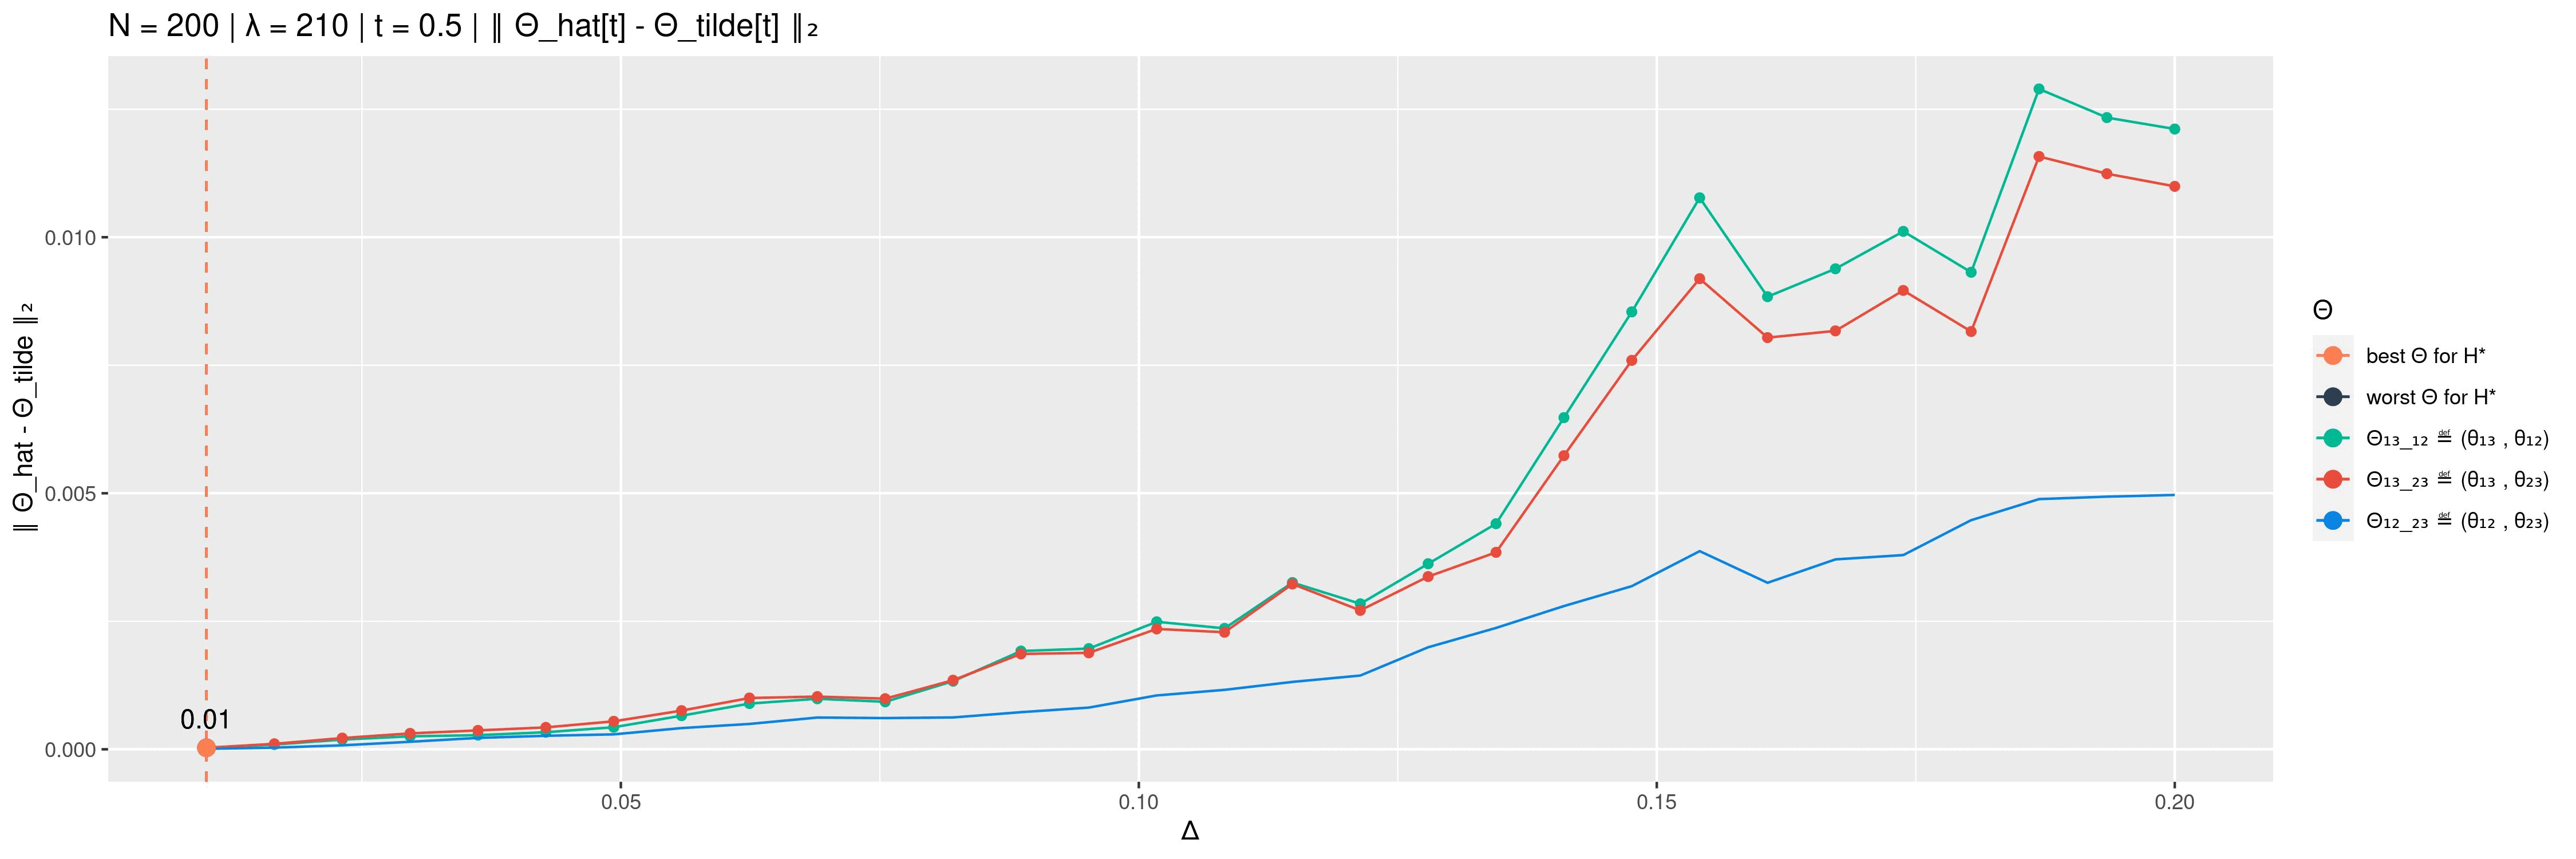
\includegraphics[width=0.8\textwidth]{Images/risque/N200_t0.5_lbd210.jpg}
\end{figure}


\begin{figure}[H]
	\centering
	\textbf{ H = 0.73 }

	Sparse :

	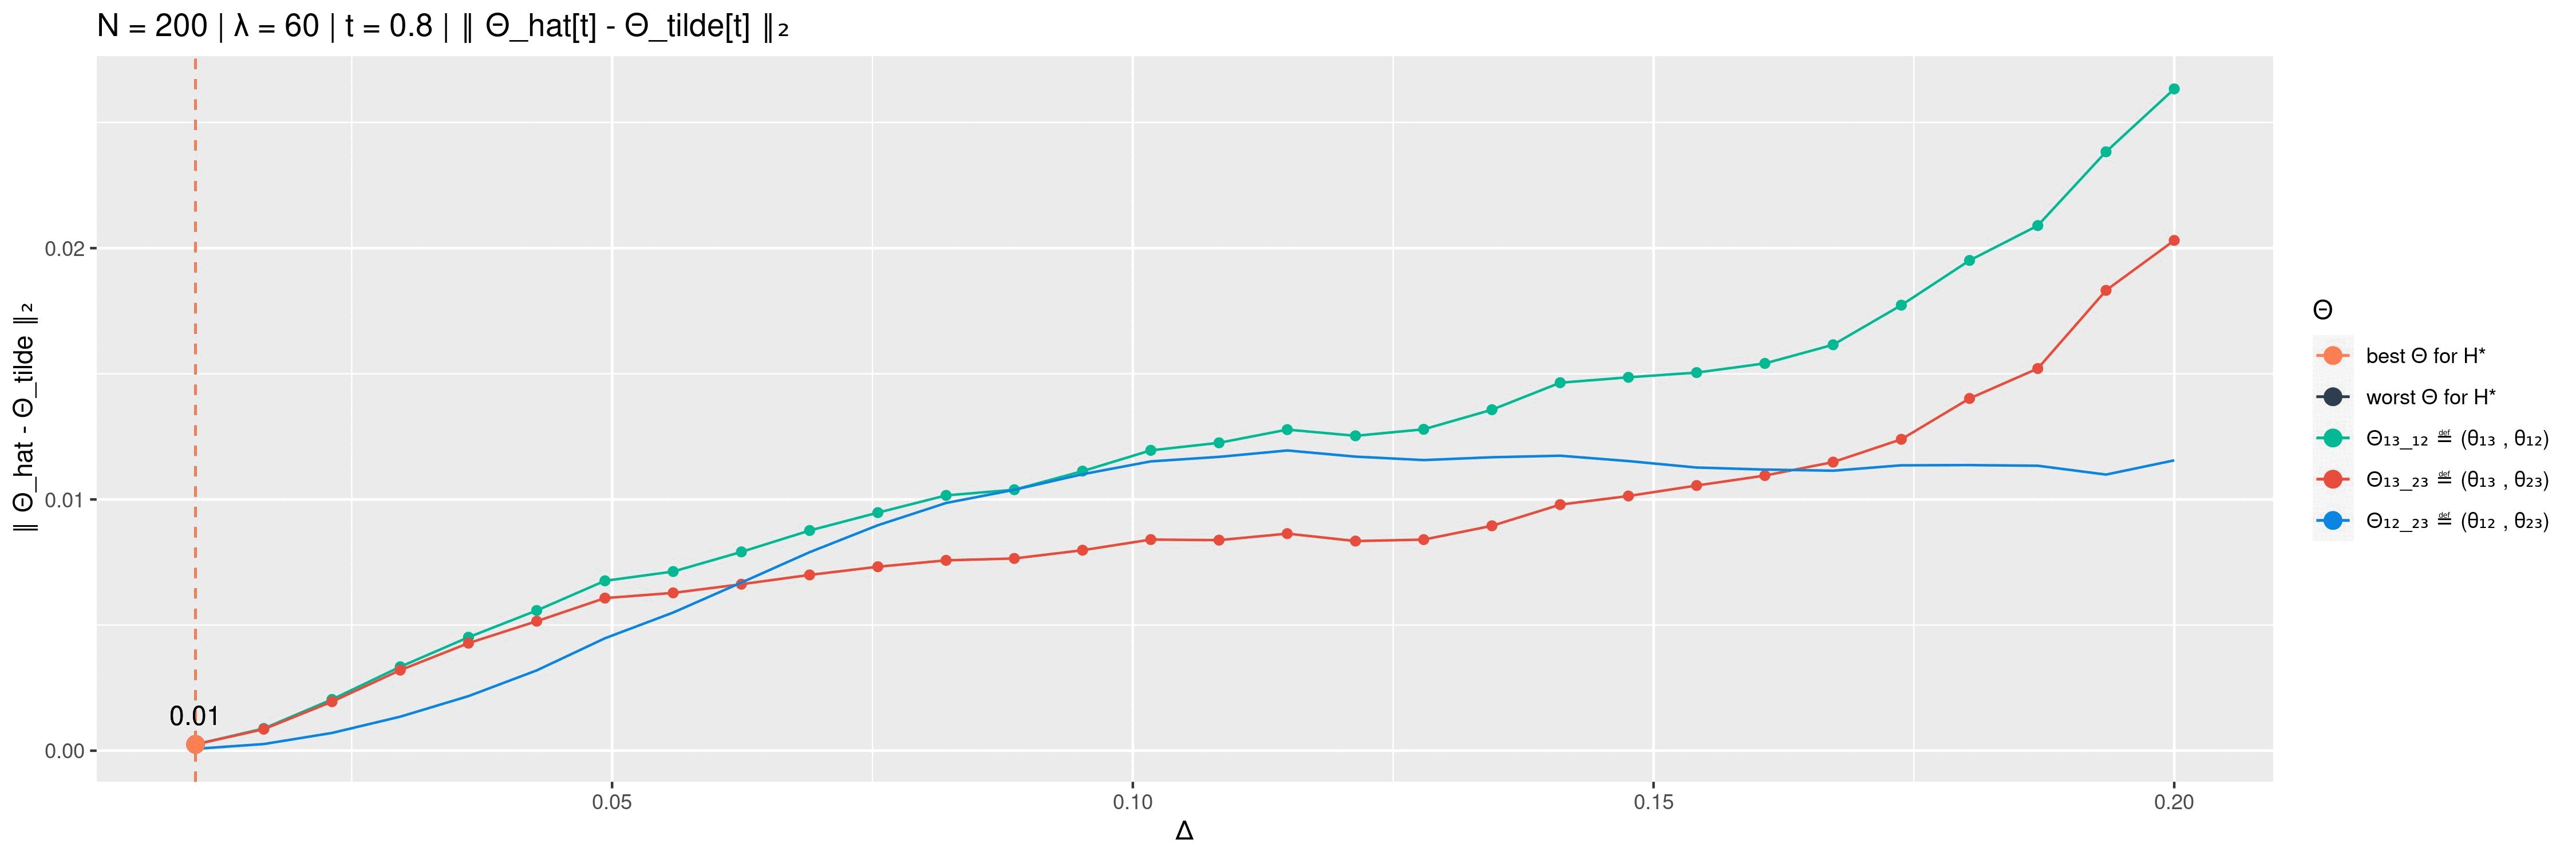
\includegraphics[width=0.8\textwidth]{Images/risque/N200_t0.8_lbd60.jpg}

	Dense :

	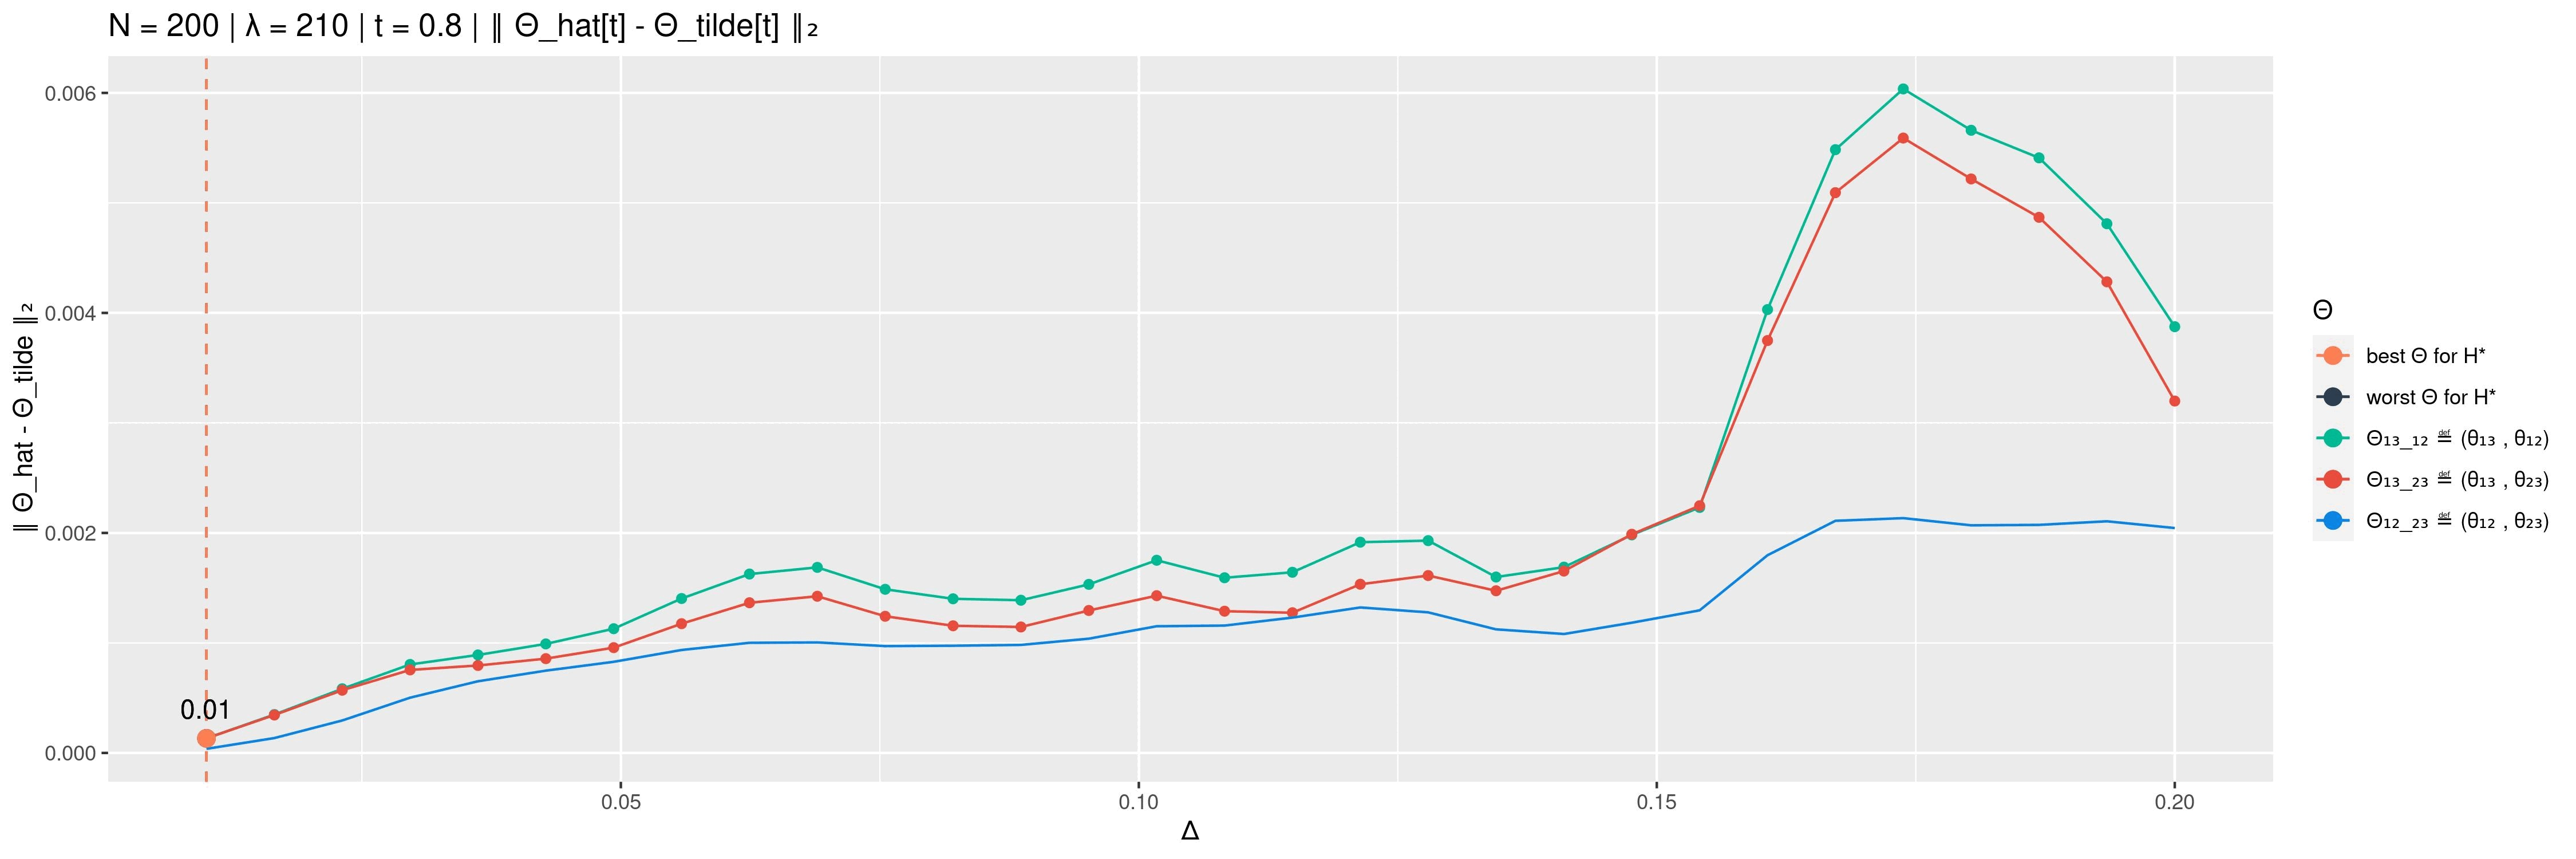
\includegraphics[width=0.8\textwidth]{Images/risque/N200_t0.8_lbd210.jpg}

	\label{fig:sparse_osef}
	\caption{Graphe des risques \textbf{euclidiens} dans les cas \og sparse \fg et \og raisonnablement dense \fg, ayant enlevé les observations extrêmes ($\leq$ 20\% des échantillons de Monte-Carlo)}
\end{figure}


%%%%		RELATIF 		%%%%

\begin{figure}[H]
	\centering
	\textbf{ H = 0.51 }

	Sparse :

	\includegraphics[width=0.8\textwidth]{Images/eucl_rel/N200_λ060_t0.3_kernel.jpg}

	Dense :

	\includegraphics[width=0.8\textwidth]{Images/eucl_rel/N200_λ210_t0.3_kernel.jpg}
\end{figure}

\begin{figure}[H]
	\centering
	\textbf{ H = 0.6 }

	Sparse :

	\includegraphics[width=0.8\textwidth]{Images/eucl_rel/N200_λ060_t0.5_kernel.jpg}

	Dense :

	\includegraphics[width=0.8\textwidth]{Images/eucl_rel/N200_λ210_t0.5_kernel.jpg}
\end{figure}

\begin{figure}[H]
	\centering
	\textbf{ H = 0.73 }

	Sparse :

	\includegraphics[width=0.8\textwidth]{Images/eucl_rel/N200_λ060_t0.8_kernel.jpg}

	Dense :

	\includegraphics[width=0.8\textwidth]{Images/eucl_rel/N200_λ210_t0.8_kernel.jpg}

	\label{fig:sparse_osef_rel}
	\caption{Graphe des \textbf{risques euclidiens relatifs} à $\widetilde \Theta(\Delta)$ dans les cas \og sparse \fg et \og raisonnablement dense \fg, ayant enlevé les observations extrêmes ($\leq$ 20\% des échantillons de Monte-Carlo)}
\end{figure}
